\lezione{6}{22.03.17}

\section{Probabilità su $\RR$}
L'insieme dei numeri reali $\RR$ è, senza troppe sorprese, un caso particolarmente importante nello studio della probabilità, e quello verso il quale sono orientate gran parte dell'attenzione e della teoria.
Ciò è dovuto innanzitutto alla comodità dell'utilizzo dei numeri (strumento ormai ben conosciuto e sviluppato) per rappresentare un generico insieme, pratica peraltro utilizzata pressoché in ogni branca della matematica.
In questo capitolo si analizzeranno le altre ragioni di questa scelta, ovvero le utili proprietà che caratterizzano $\RR$ e la possibilità di introdurre nuovi strumenti di calcolo, tra loro legati: la \emph{funzione di ripartizione}, che ``raccoglie'' la probabilità totale al crescere del suo argomento, e la \emph{densità di probabilità}, che descrive il peso di ogni singolo punto di $\RR$ nel determinare la probabilità di un evento.
Saranno infine forniti alcuni esempi notevoli di distribuzioni molto usate nello studio della materia.

\subsection{Funzione di ripartizione}
Per ricapitolare i teoremi dei capitoli precedenti:
\begin{enumerate}
  \item per generare $\Ac$: è sufficiente definire $\Cc \subset \Ac$ tale che $\sigma(\Cc) = \Ac$;
  \item per caratterizzare $\PP$ su $\Ac$: è sufficiente definire $\Cc \subset \Ac$ tale che $\sigma(\Cc) = \Ac $ con $ \Cc$ chiuso per intersezioni finite;
  \item per costruire $\PP$ su $\Ac$: è sufficiente definire $\Cc \subset \Ac$ tale che $\sigma(\Cc) = \Ac$ con $\Cc$ algebra.
\end{enumerate}

\begin{defn}
  \index{funzione!di ripartizione}
  Sia $(\Omega, \Ac) = (\RR, \Bc)$ e sia $\PP: \Bc \to [0,1]$ una probabilità su $\Bc$. \\
  La \textbf{funzione di ripartizione} di $\PP$ è definita come:
  $$ F: \RR \to [0,1], \ \
  F(x) \coloneqq \PP( \left( -\infty,x \right] ).
  $$
\end{defn}
\vskip\medskipamount
\begin{teob}[\JPTh{7.1}]
  \label{teo-prob-ripartizione}
  Siano $\PP$ probabilità su $(\RR, \Bc)$ e $F$ funzione di ripartizione,
  allora $F$ caratterizza $ \PP $, ovvero dati $\PP_1$ e $\PP_2$ probabilità su $\Bc$ allora:
  $$\PP_1 = \PP_2 \iff F_1 = F_2$$
\end{teob}
\begin{dimo}
  La dimostrazione di ($\implies$) è ovvia. \\
  Dimostriamo ($\impliedby$):
  Sia $\Cc = \{(-\infty, q], q \in \QQ\}$. Abbiamo già dimostrato che $\sigma(\Cc) = \Bc$.

  Mostriamo che $\Cc$ è chiuso per intersezioni finite: \\
  $$\underbrace{(-\infty, q_1]}_{\in \, \Cc} \ \cap \ \underbrace{(-\infty, q_2]}_{\in \ \Cc} = \underbrace{(-\infty, \min(q_1, q_2)]}_{\in \ \Cc}\\$$
  Allora:
  \begin{align*}
    F_1 = F_2 &\iff F_1(x) = F_2(x) \quad \forall x \in \RR \\
    & \, \implies F_1(q) = F_2(q) \quad \forall q \in \QQ\\
    &\iff \PP_1((-\infty, q]) = \PP_2((-\infty, q]) \quad \forall q \in \QQ\\
    &\iff \PP_1(B) = \PP_2(B) \quad \forall B \in \Cc\\
    &\iff \PP_1 = \PP_2 \text{ su } B \in \sigma(\Cc)
  \end{align*}
  Abbiamo usato il corollario \ref{coro-estensione-prob} delle classi monotone. \qedhere

\end{dimo}
\subsubsection{Caratterizzazione}
\begin{teob}[\JPTh{7.2}]
  $F:\RR \to [0,1]$ è funzione di ripartizione di una (e una sola) probabilità $\PP:\Bc \to [0,1]$ se e solo se:
  \begin{enumerate}
    \item $F$ è non-decrescente;
    \item $F$ è continua da destra;
    \item $\lim\limits_{x \to -\infty} F(x) = 0, \quad \lim\limits_{x \to +\infty} F(x) = 1$.
  \end{enumerate}
\end{teob}

\begin{dimo}
  Dimostriamo ($\implies$):
  \begin{enumerate}
    \item $F$ è non-decrescente: $x_1 < x_2 \implies F(x_1) \leq F(x_2)$ \\*
      Infatti, poiché $(-\infty, x_1] \subseteq (-\infty, x_2]$, per il corollario \ref{coro-definizione-prob} si ha:
      $$F(x_1) = \PP((-\infty, x_1]) \leq \PP((-\infty, x_2]) = F(x_2)$$
    \item $F$ continua da destra: $\forall x, \quad \forall x_n \downarrow x \quad F(x) = \lim_{n} F(x_n)$\\*
      Infatti:
      $$(-\infty, x_n] \supseteq (-\infty, x_{n+1}] \implies (-\infty, x_n) \downarrow \bigcap\limits_n (-\infty, x_n] = (-\infty, x]$$
      Per dimostrare l'ultima uguaglianza basti osservare che
      $$y \in \bigcap\limits_n \, (-\infty, x_n] \implies y \in (-\infty, x_n] \ \forall n$$
      Allora, $y \leq x_n \  \forall n$ e dunque, per il teorema dei due carabinieri, $y \leq x \leq x_n$. \\
      Infine:
      $$F(x_n) = \PP((-\infty, x_n]) \downarrow \PP((-\infty, x]) = F(x)$$
    \item $\lim\limits_{x \to -\infty} F(x) = 0, \quad \lim\limits_{x \to +\infty} F(x) = 1$:
      \begin{enumerate}
        \item $x_n \downarrow -\infty \implies (-\infty, x_n] \downarrow \varnothing \implies$
          $F(x_n) = \PP((-\infty, x_n]) \downarrow \PP(\varnothing) = 0$
        \item $x_n \uparrow +\infty \implies (-\infty, x_n] \uparrow \RR \implies$
          $F(x_n) = \PP((-\infty, x_n]) \uparrow \PP(\RR) = 1$
      \end{enumerate}
  \end{enumerate}
  \medskip

  Dimostriamo ($\impliedby$)\footnote{Fuggite sciocchi, finché siete in tempo}:

  Sia $ F: \RR \to [0,1]$ che soddisfa (1), (2), (3).\\
  Definiti inoltre:
  $$\Bc_0 = \left \{ B= \bigcup_{k=1}^n (x_k, y_k] | n \in \NN, \ -\infty \le x_1 \le y_1 \le x_2 \le y_2 \le \dots \le +\infty \right \}$$
  e $\PP_0$ tale che:
  $$\PP_0: \Bc_0 \to [0,1], \quad \PP_0 \left( \bigcup_{k=1}^n ( x_k, y_k ] \right) = \sum_{k=1}^{n} \left[ F(y_k) - F(x_k) \right]$$
  dove $F(-\infty)=0$ e $F(+\infty)=1$
  \begin{enumerate}   \renewcommand{\labelenumi}{\alph{enumi})}
    \item $\PP_0$ è ben definita, perché $\PP_0( ( a, a] )= 0$ e $ \PP_0( (a, b] \cup (b, c] ) = F(c) -F(a)$
    \item $\PP_0 (\RR) =1$ perché
        $$\PP_0( \RR) = \PP_0( (-\infty, +\infty) )= \PP_0 ( (-\infty, +\infty] )= F({+\infty}) - F(-\infty) = 1-0=1$$
    \item $\PP_0$ è $\sigma$-additiva su $\Bc_0$.\\
        Poiché $\PP_0$ è additiva, $\PP_0$ risulta $\sigma$-additiva se e solo se $\PP_0(A_n) \downarrow 0 \forall$ successione tale che:
        $$A_n \in \Bc_0, \ A_n \downarrow \varnothing, \ \ A_l = \bigcup_{k=1}^{n_l} ( x_k^l, \ y_k^l]$$
        $$\text{dove } -\infty \le x_1^l < y_1^l < x_2^l < \dots < y_{n_l}^l \le +\infty \ \text{ e } \ A_1 \supseteq A_2 \supseteq A_3 \dots$$
        Vorremmo passare a dei nuovi insiemi $\widebar{B}_l$ compatti, approssimando $A_l$, dove $\widebar{B}_l \downarrow \varnothing \implies \widebar{B}_l = \varnothing$ definitivamente $\implies \PP_0( \widebar{B}_l)=0$ definitivamente.
  \end{enumerate}
  Fissato $\varepsilon >0 $ si mostra che $\exists \Lc = \Lc (\varepsilon)$ tale che $ \PP_0(A_l) \le 3 \varepsilon \ \forall l > \Lc.$\\
  \begin{enumerate}
    \item Si trova $z$ tale che $F(-z) \le \varepsilon$ e $1-F(z) \le \varepsilon$ ovvero $\PP_0( (-z, z]^C ) \le 2 \varepsilon.$\\
      Allora si può mostrare che:
      $$
      \lim_{x \to -\infty} F(x) =0 \implies \exists \, z_1 \text{ t.c. } F(x) \le \varepsilon \ \forall x \le z_1
      $$
      $$
      \lim_{x \to +\infty} F(x) =1 \implies \exists \, z_2  \text{ t.c. } F(x) \ge 1 - \varepsilon \ \forall x \ge z_2$$
      Prendiamo quindi il massimo\footnote{Si noti la notazione alternativa per il massimo tra due elementi. Similmente, per il minimo tra due elementi $x$ e $y$ si scriverà $\max \left \{ x, \, y \right \} = x \land y$.} dei due valori:
      $$z= \max \left \{ |z_1|, \ |z_2| \right \} = |z_1| \lor |z_2| \implies F(-z) \le \varepsilon \ F(z) \ge 1 - \varepsilon$$
      Allora:
      \begin{align*}
        \PP_0(A_l) &= \PP_0( A_l \land (-z, z]^C ) + \PP_0( A_l \land (-z, +z] ) \\
        &\le \PP_0 \left( (-z, z]^C \right) + \PP_0 \left( A_l, (-z,z] \right) \\
        &\le 2 \varepsilon + \PP_0 \left( A_l, (-z,z] \right)
      \end{align*}

    \item $\forall l \in \NN, \ \forall k=1, \dots , n_l \ \exists a_k^l \in (x_k^l, y_k^l)$ tale che $F(a_k^l) - F(x_k^l) \le \dfrac{\varepsilon}{2^{l+k}}$ per la proprietà 2.

    \item Possiamo quindi trovare dei $B_l'$ che:
      $$B_l' = \left( \bigcup_{k=1}^{n_l} (a_k^l, y_k^l) \right) \cap (-z,z] \ \text{ con } B_l' \in \Bc_0, \ B_l' \in A_l, \ \widebar{B}_l' \subseteq A_l , \ \widebar{B}_l' \subseteq [-z, z]$$
      Allora:
      \begin{align*}
        \PP_0(A_l \ \setminus \ \widebar{B}_l') &\le 2 \varepsilon + \PP_0 ( (A_l \ \setminus \ B_l' ) \cap [-z, z] ) \\[4pt]
        &\le 2 \varepsilon + \PP_0 \left( \bigcup_{k=1}^{n_l} [x_k^l, y_k^l] \ \mathbin{\Big\backslash} \, \bigcup_{k=1}^{n_l} [a_k^l, y_k^l] \right) & (\text{per definizione})\\[2pt]
        &\le 2 \varepsilon + \PP_0 \left( \bigcup_{k=1}^{n_l} [x_k^l, a_k^l] \right) \\[2pt]
        &= 2\varepsilon+ \sum_{k=1}^{n_l} \PP_0( [x_k^l, a_k^l]) & (\text{per $\sigma$-additività})\\
        &= 2 \varepsilon + \sum_{k=1}^{n_l} ( F(a_k^l) - F(x_k^l ) ) & (\text{per le prop. di } F)
      \end{align*}
      Passando ai $B_l'$:
      \begin{align*}
        \PP_0 (A_l \ \setminus \ B_l') &\le 2 \varepsilon + \sum_{k=1}^{n_l} \dfrac{\varepsilon}{2^{l+k}} & (\text{sfruttando il punto (2)})\\
        &\le 2 \varepsilon + \dfrac{\varepsilon}{2^l} \sum_{n=1}^{+\infty} \dfrac{1}{2^n}  & (\text{serie a termini positivi})\\
        &\le \left( 2+ \dfrac{1}{2^l} \right) \varepsilon & (\text{la sommatoria vale 1})
      \end{align*}
      Tuttavia i $B_l'$ non sono inscatolati.

    \item Sia:
      $$B_l = \bigcap_{m=1}^l B_m' \implies B_l \in \Bc_0, \ B_l \in B_l' \subseteq A_l, \ \widebar{B}_l \subseteq \bigcap_{m=1}^{+\infty} \widebar{B}_m' \subseteq \widebar{B}_l' \subseteq A_l $$
      Allora possiamo mostrare che $B_l \supseteq B_{l+1} \text{ e } \bigcap_l B_l \subseteq \bigcap_l A_l = \varnothing \implies B_l \downarrow \varnothing$, quindi analogamente $\widebar{B}_l \downarrow \varnothing$\\
      A questo punto, la differenza tra $A_l$ e $B_l$:
      \begin{align*}
        A_l \ \setminus \ B_l &= A_l \cap B_l^C = A_l \cap \left( \bigcap_{m=1}^l B_m' \right)^C \\
        &= A_l \cap \left(\bigcup_{m=1}^l {B'_m}^C \right) = \bigcup_{m=1}^l \left( A_l \cap {B_l'}^C \right)\\
        &\subseteq \bigcup_{m=1}^l \left( A_m \cap {B_m'}^C \right) = \bigcup_{m=1}^l \left(A_m \ \setminus \ B_m'\right)
      \end{align*}
      dove per l'inclusione si è usato il fatto che gli $A_l$ sono inscatolati.
      Possiamo quindi concludere che:
      \begin{align*}
        \PP_0( A_l \ \setminus \ B_l) &\le \PP_0 \left( \bigcup_{m=1}^l (A_m \ \setminus \ B_m' ) \right) \\
        &\le \sum_{m=1}^l \PP_0 \left( A_m \ \setminus \ B_m'\right) & (\text{per subadditività})\\
        &\le 2 \varepsilon + \PP_0 \left( \bigcup_{m=1}^l \left(A_m \ \setminus \ B_m' \right) \cap (-z,z] \right) & (\text{analogamente a (3)})\\
        &\le 2 \varepsilon + \sum_{m=1}^l \PP_0  \left( \left(A_m \ \setminus \ B_m' \right) \cap (-z,z] \right) & (\text{per $\sigma$-additività})\\
        &= 2 \varepsilon + \dfrac{\varepsilon}{2^l} \le 3 \varepsilon & (\text{analogamente a (3)})
      \end{align*}

    \item $\exists \, \Lc$ tale che $B_l = \varnothing \ \forall l \ge \Lc $. Infatti, i $\widebar{B}_l$ sono compatti e
      $\widebar{B}_l \downarrow \varnothing$: se per assurdo esistesse $ l_j$ tale che $\widebar{B}_{l_j} \ne \varnothing$, si avrebbe $\forall j \ l_j \to +\infty$ allora $\exists b_j \in \widebar{B}_{l_j} \ \forall j \to b_j \in [-z, z] \ \forall j $.

      Quindi, per le proprietà dei compatti, $\exists \, b_{ji} \stackrel{i}{\to} b \in [-z, z]$, ma $b \in \widebar{B}_l \ \forall l$ essendo $b_j \in \widebar{B}_l$ definitivamente, $\widebar{B}_l$ compatti allora $\cap_l \widebar{B}_l \ni b$.
      Quest'ultima affermazione è un assurdo, quindi $\widebar{B}_l = \varnothing$ e $B_l = \varnothing$ entrambe definitivamente.

    \item Visti i risultati dei passaggi precedenti si può affermare che:
      \begin{align*}
        \PP_0(A_l) &= \PP_0(A_l) - \PP_0(B_l) + \PP_0(B_l) & (\text{aggiungendo e togliendo } \PP_0(B_l))\\
        &= \PP_0( A_l \ \setminus \ B_l) + \PP_0(B_l) \\
        &= \PP_0(A_l \ \setminus \ B_l) \le 3 \varepsilon &  (\text{se $l \ge \Lc$ allora $\PP_0(B_l) =0$})
      \end{align*}
      Questo conclude la dimostrazione. \qedhere
  \end{enumerate}
\end{dimo}

\lezione{7}{23.03.17}

\subsubsection{Proprietà}
Introduciamo la notazione $F(x^-) \coloneqq \lim\limits_{y \, \uparrow \, x} F(y)$.
Sicuramente $F(x^-) \le F(x)$.

\begin{coro}
  Sia $F$ funzione di ripartizione di $\PP$ su $(\RR, \Bc)$.
  Allora, $\forall x < y$:
  \begin{enumerate}
  \item $\PP((x, y]) = F(y) - F(x)$
  \item $\PP([x, y]) = F(y) - F(x^-)$
  \item $\PP((x, y)) = F(y^-) - F(x)$
  \item $\PP([x, y)) = F(y^-) - F(x^-)$
  \item $\PP(\{ x \}) = F(x) - F(x^-)$
  \end{enumerate}
\end{coro}

\begin{dimo}
  \leavevmode\vspace{-\baselineskip}
  \begin{enumerate}
  \item Per costruzione.
  \item
    $[x, y] = \bigcap\limits_{n=1}^{+\infty} \left(x - \dfrac 1 n, y \right]$. Dunque: \\
    \begin{align*}
    \PP([x, y])
    &= \lim\limits_{n \to +\infty}
    \PP \left( \left(x - \dfrac 1 n, y \right] \right) \\
    &= \lim\limits_{n \to +\infty}
    \left( F(y) - F \left( x - \dfrac 1 n \right) \right)
    = F(y) - F(x^-)
    \end{align*}
  \end{enumerate}
  Analogamente si verificano i punti (3), (4), (5).
\end{dimo}

\vskip\bigskipamount
\begin{defn}\label{def-delta-dirac}
  \index{delta di Dirac}
  Si definisce massa o \textbf{delta di Dirac} in $\alpha$ (indicata con $\delta_\alpha$) la probabilità così definita:
  $$
  \PP(A)
  = \begin{cases}
    1 & \text{se } \alpha \in A \\
    0 & \text{se } \alpha \not\in A
    \end{cases}
  \qquad \text{con } \alpha \in \RR, A \in 2^\RR
  $$

  La sua funzione di ripartizione è:
  $$
  F(x) = \PP((-\infty, x])
  = \begin{cases}
    1 & \text{se } x \ge \alpha \\
    0 & \text{se } x < \alpha
    \end{cases}
  $$
  \begin{figure}[H]
  \centering
  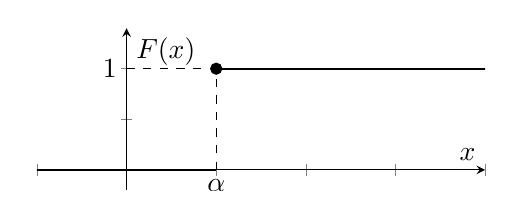
\begin{tikzpicture}
    \begin{axis}[
      axis lines = middle,
      ylabel = $F(x)$,
      xlabel = $x$,
      width=0.6\textwidth,
      height=0.3\textwidth,
      yticklabels={,,},
      xticklabels={,,}
    ]
    \draw [line width=0.1mm, dashed] (axis cs:0,1) -- (axis cs:1,1) -- (axis cs:1,0);

    \draw [line width=0.3mm] (axis cs:-2,0) -- (axis cs:1,0);
    \draw [line width=0.3mm] (axis cs:1,1) -- (axis cs:5,1);

    \addplot [only marks, mark=*] table {
    1 1
    };

    \addplot [draw=none, forget plot] coordinates {(-1,-0.2)};
    \addplot [draw=none, forget plot] coordinates {(4,1.4)};
    \addplot [draw=none, forget plot] coordinates {(1,0)} node[below] {$\alpha$};
    \addplot [draw=none, forget plot] coordinates {(0,1)} node[left] {$1$};

    \end{axis}
  \end{tikzpicture}

  \caption{funzione di ripartizione della delta di Dirac}
  \end{figure}
\end{defn}
\begin{nb}
  Questa distribuzione è un caso degenere e verrà spesso utilizzata per i limiti di variabili aleatorie, quando queste tendono ad avere varianza nulla.
\end{nb}

\begin{ese}
  Sia data $\PP$ probabilità discreta sui punti $x_k \ (k \in \NN)$
  con la seguente densità:
  $$p_j \ge 0 \text{ tale che }\sum\limits_{k=1}^{+\infty} p_k = 1$$
  Per $A \in 2^\RR$, ovvero non restringendo il campo ai soli boreliani:
  $$\PP(A) \coloneqq \sum\limits_{k: \, x_k \in A} p_k, \text{ da cui } F(x) \coloneqq \sum\limits_{k: \, x_k \le x} p_k$$

  Il grafico della $F(x)$ sarà \textit{a scala}, presentando discontinuità di tipo salto
  in corrispondenza delle $x_k$.

  \begin{figure}[H]
  \centering
  \begin{tikzpicture}
    \begin{axis}[
      axis lines = middle,
      ylabel = $F(x)$,
      xlabel = $x$,
      width=0.7\textwidth,
      height=0.4\textwidth
    ]

    \draw [line width=0.3mm] (axis cs:-2,0) -- (axis cs:-0.5,0);
    \draw [line width=0.3mm] (axis cs:-0.5,0.2) -- (axis cs:0.75,0.2);
    \draw [line width=0.3mm] (axis cs:0.75,0.5) -- (axis cs:2,0.5);
    \draw [line width=0.3mm] (axis cs:2,0.6) -- (axis cs:3,0.6);
    \draw [line width=0.3mm] (axis cs:3,1) -- (axis cs:5,1);
    \draw [line width=0.1mm, dashed] (axis cs:0,1) -- (axis cs:3,1);

    \addplot [only marks, mark=*] table {
    -0.5 0.2
    0.75 0.5
    2 0.6
    3 1
    };

    \addplot [draw=none, forget plot] coordinates {(-1,-0.2)};
    \addplot [draw=none, forget plot] coordinates {(4,1.4)};

    \end{axis}
  \end{tikzpicture}

  \caption{funzione di ripartizione di una variabile aleatoria discreta}
  \end{figure}
\end{ese}

\textit{Esempi di probabilità discrete}:
\begin{itemize}
  \item binomiale ($\PP = B(n, p)$, con
  $n \in \NN, \enspace 0 \le p \le 1$);
  \item Poisson ($\PP = Po(\lambda)$, con
  $\lambda \in \RR$).
\end{itemize}

\subsection{Densità continua di probabilità}
\begin{defn}
  \index{densità di probabilità!continua}
  Si dice \textbf{densità continua di probabilità} una $f: \RR \to [0, +\infty)$, non negativa, Riemann-integrabile e tale che:
  $$\int_{-\infty}^{+\infty} f(x) \, \dx = 1$$

  Si dice inoltre che \textit{$F$ ammette densità $f$} se vale:
  $$F(x) = \int_{-\infty}^{x} f(t) \, \de t$$
\end{defn}

Osserviamo che, se $F$ ammette densità $f$, $F'(x) = f(x) \enspace \forall x$ e $F \in C^0$, quindi ogni punto ha probabilità zero:
$$\PP(\{x\}) = 0 \enspace \forall x \in \RR$$
Vedremo più avanti che i punti sono \textit{insiemi di misura trascurabile} rispetto agli insiemi non numerabili. \\
Se $f \in C^0$ a tratti, allora $F \in C^1$ a tratti. Inoltre, se $F \in C^0, \ C^1$ a tratti, $F$ ammette densità e $f(x) = F'(x)$
per ogni $x$ in cui $F$ è derivabile (i punti di non derivabilità non influenzano $f$).

Sia poi $\PP$ la probabilità su $(\RR, \Bc)$ associata a $F$, allora:
$$\PP((a, b)) = \PP([a, b]) = \int_{a}^{b} f(t) \, \de t = \int_{-\infty}^{b} f(t) \, \de t - \int_{-\infty}^{a} f(t) \, \de t$$

\begin{figure}[H]
  \centering
  \begin{tikzpicture}
  \tikzset{
    hatch distance/.store in=\hatchdistance,
    hatch distance=5pt,
    hatch thickness/.store in=\hatchthickness,
    hatch thickness=0.5pt
  }

  \begin{axis}[
    axis lines = middle,
    ylabel = $f(x)$,
    xlabel = $x$,
    width=0.7\textwidth,
    height=0.4\textwidth,
    yticklabels={,,},
    xticklabels={,,}
  ]

  \draw [line width=0.3mm] (axis cs:-2,0) -- (axis cs:-0.7,0);
  \addplot [only marks, mark=*] table {
    -0.7 0
    };

  \addplot[color=black,
    domain=-0.7:4,
    samples=100,
    line width=0.3mm] {1/sqrt(2*pi)*exp(-x^2/2)};
  \addplot+[mark=none,
    domain=-0.7:-0.2,
    samples=100,
    pattern=flexible hatch,
    area legend,
    draw=black,
    pattern color=lightgray]{1/sqrt(2*pi)*exp(-x^2/2)} \closedcycle;

  \addplot [draw=none, forget plot] coordinates {(-0.7,-0.05)} node {$a$};
  \addplot [draw=none, forget plot] coordinates {(-0.2,-0.045)} node {$b$};

  \addplot [draw=none, forget plot] coordinates {(-1.5,-0.1)};
  \addplot [draw=none, forget plot] coordinates {(0,0.5)};

  \end{axis}
  \end{tikzpicture}

  \caption{probabilità di un evento caratterizzato da $f \in C^0$ a tratti. L'area tratteggiata rappresenta $\PP(a,b)$}
\end{figure}

\subsubsection{Densità notevoli}
Si rimanda alle appendici B e C a pagina \pageref{appendice-discrete} e \pageref{appendice-continue} per una lista più completa delle densità notevoli.
\begin{itemize}
  \item \textbf{Distribuzione uniforme}:
  \index{distribuzione!uniforme}
  \begin{gather*}
    \PP = U([a, b]),
    \quad f(s) = \dfrac 1 {b - a} \ \Ind_{[a, b]}(s)
  \end{gather*}
  \begin{figure}[H]
    \centering
    \begin{tikzpicture}
    \begin{axis}[
      axis lines = middle,
      ylabel = $f(x)$,
      xlabel = $x$,
      width=0.7\textwidth,
      height=0.4\textwidth,
      yticklabels={,,},
      xticklabels={,,}
    ]

    \draw [line width=0.3mm] (axis cs:-2,0) -- (axis cs:1,0);
    \draw [line width=0.3mm] (axis cs:1,1) -- (axis cs:3,1);
    \draw [line width=0.3mm] (axis cs:3,0) -- (axis cs:5,0);
    \draw [line width=0.1mm, dashed] (axis cs:0,1) -- (axis cs:1,1);

    \addplot [only marks, mark=*] table {
    1 1
    3 1
    };

    \addplot [draw=none, forget plot] coordinates {(-1,-0.2)};
    \addplot [draw=none, forget plot] coordinates {(4,1.4)};

    \addplot [draw=none, forget plot] coordinates {(0,1)} node[left] {$\frac{1}{b-a}$};
    \addplot [draw=none, forget plot] coordinates {(1,0)} node[below] {$a$};
    \addplot [draw=none, forget plot] coordinates {(3,0)} node[below] {$b$};

    \end{axis}
    \end{tikzpicture}
    \caption{densità uniforme}
  \end{figure}
  \begin{figure}[H]
    \centering
    \begin{tikzpicture}
    \begin{axis}[
      axis lines = middle,
      ylabel = $F(x)$,
      xlabel = $x$,
      width=0.7\textwidth,
      height=0.4\textwidth,
      yticklabels={,,},
      xticklabels={,,}
    ]

    \draw [line width=0.3mm] (axis cs:-2,0) -- (axis cs:1,0);
    \draw [line width=0.3mm] (axis cs:1,0) -- (axis cs:3,1);
    \draw [line width=0.3mm] (axis cs:3,1) -- (axis cs:5,1);
    \draw [line width=0.1mm, dashed] (axis cs:0,1) -- (axis cs:3,1);

    \addplot [draw=none, forget plot] coordinates {(-1,-0.2)};
    \addplot [draw=none, forget plot] coordinates {(4,1.4)};

    \addplot [draw=none, forget plot] coordinates {(0,1)} node[left] {$1$};
    \addplot [draw=none, forget plot] coordinates {(1,0)} node[below] {$a$};
    \addplot [draw=none, forget plot] coordinates {(3,0)} node[below] {$b$};

    \end{axis}
    \end{tikzpicture}

    \caption{funzione di ripartizione uniforme}
  \end{figure}
  \item \textbf{Distribuzione esponenziale}:
  \index{distribuzione!esponenziale}
  \begin{gather*}
    \PP = \Ec(\lambda),
    \quad f(s) = \lambda \ e^{-\lambda s} \ \Ind_{[0, +\infty)}(s),
    \quad F(s) = \left( 1 - e^{-\lambda s} \right) \ \Ind_{[0, +\infty)}(s)
  \end{gather*}
  \begin{figure}[H]
    \centering
    \begin{tikzpicture}
    \begin{axis}[
      axis lines = middle,
      ylabel = $f(x)$,
      xlabel = $x$,
      width=0.7\textwidth,
      height=0.4\textwidth,
      yticklabels={,,},
      xticklabels={,,}
    ]

    \draw [line width=0.3mm] (axis cs:-2,0) -- (axis cs:0,0);

    \addplot [only marks, mark=*] table {
    0 1
    };

    \addplot [
      domain=0:5,
      samples=100,
      color=black,
      line width=0.3mm
      ]
      {e^(-x)};

    \addplot [draw=none, forget plot] coordinates {(-1,-0.2)};
    \addplot [draw=none, forget plot] coordinates {(4,1.4)};

    \addplot [draw=none, forget plot] coordinates {(0,1)} node[left] {$\lambda$};

    \end{axis}
    \end{tikzpicture}
  \caption{densità esponenziale}
  \end{figure}
  \begin{figure}[H]
    \centering
    \begin{tikzpicture}
    \begin{axis}[
      axis lines = middle,
      ylabel = $F(x)$,
      xlabel = $x$,
      width=0.7\textwidth,
      height=0.4\textwidth,
      yticklabels={,,},
      xticklabels={,,}
    ]

    \draw [line width=0.3mm] (axis cs:-2,0) -- (axis cs:0,0);
    \draw [line width=0.1mm, dashed] (axis cs:0,1) -- (axis cs:5,1);

    \addplot [
      domain=0:5,
      samples=100,
      color=black,
      line width=0.3mm
      ]
      {1-e^(-x)};

    \addplot [draw=none, forget plot] coordinates {(-1,-0.2)};
    \addplot [draw=none, forget plot] coordinates {(4,1.4)};

    \addplot [draw=none, forget plot] coordinates {(0,1)} node[left] {$1$};


    \end{axis}
    \end{tikzpicture}

    \caption{funzione di ripartizione esponenziale}
  \end{figure}
  \item \textbf{Distribuzione gaussiana} o \textbf{normale}:
  \index{distribuzione!gaussiana}
  \index{distribuzione!normale}
  \begin{gather*}
    \PP = N(\mu, \sigma^2),
    \quad f(s) = \dfrac 1 {\sqrt{2\pi\sigma^2}} \,
    \exp \left\{ - \dfrac {(s - \mu) ^ 2} {2 \sigma^2} \right\}
  \end{gather*}
  \begin{figure}[H]
    \centering
    \begin{tikzpicture}
    \begin{axis}[
      axis lines = middle,
      ylabel = $f(x)$,
      xlabel = $x$,
      width=0.7\textwidth,
      height=0.4\textwidth,
      yticklabels={,,},
      xticklabels={,,}
    ]

    \addplot [
      domain=-3:5,
      samples=100,
      color=black,
      line width=0.3mm
      ]
      {1/sqrt(2*pi)*e^(-(x-1)^2/2};

    \addplot [draw=none, forget plot] coordinates {(1, 0.5)};

    \end{axis}
    \end{tikzpicture}
    \caption{densità gaussiana}
  \end{figure}
  \begin{figure}[H]
    \centering
    \begin{tikzpicture}[
    declare function={erf(\x)=%
      (1+(e^(-(\x*\x))*(-265.057+abs(\x)*(-135.065+abs(\x)%
      *(-59.646+(-6.84727-0.777889*abs(\x))*abs(\x)))))%
      /(3.05259+abs(\x))^5)*(\x>0?1:-1);},
    declare function={erf2(\x,\y)=erf(\x)+erf(\y);}
    ]
    \begin{axis}[
      axis lines = middle,
      ylabel = $F(x)$,
      xlabel = $x$,
      width=0.7\textwidth,
      height=0.4\textwidth,
      yticklabels={,,},
      xticklabels={,,}
    ]

    \draw [line width=0.1mm, dashed] (axis cs:0,1) -- (axis cs:5,1);

    \addplot [
      domain=-3:5,
      samples=100,
      color=black,
      line width=0.3mm
      ]
      {1/2*(1+erf((x-1)/sqrt(2)))};

    \addplot [draw=none, forget plot] coordinates {(1, 1.2)};
    \addplot [draw=none, forget plot] coordinates {(0,1)} node[left] {$1$};

    \end{axis}
    \end{tikzpicture}
    \caption{funzione di ripartizione gaussiana}
  \end{figure}
\end{itemize}

\begin{nb}
  Per ammettere densità la funzione di ripartizione deve essere continua, essendo il risultato di un'integrazione.
  \begin{figure}[H]
  \centering
  \begin{tikzpicture}
    \begin{axis}[
      axis lines = middle,
      ylabel = $F(x)$,
      xlabel = $x$,
      width=0.7\textwidth,
      height=0.4\textwidth,
      yticklabels={,,},
      xticklabels={,,}
    ]

    \draw [line width=0.3mm] (axis cs:-2,0) -- (axis cs:1,0);
    \draw [line width=0.1mm, dashed] (axis cs:0,1) -- (axis cs:5,1);

    \addplot [only marks, mark=*] table {
    1 0.632120
    };

    \addplot [
      domain=1:5,
      samples=100,
      color=black,
      line width=0.3mm
      ]
      {1-e^(-x)};

    \addplot [draw=none, forget plot] coordinates {(-1,-0.2)};
    \addplot [draw=none, forget plot] coordinates {(4,1.4)};

    \addplot [draw=none, forget plot] coordinates {(0,1)} node[left] {$1$};

    \end{axis}
  \end{tikzpicture}
  \caption{funzione di ripartizione che non ammette densità}
  \end{figure}
\end{nb}

\cleardoublepage
